\documentclass[a4paper]{article}

%\usepackage[english]{babel}
\usepackage[utf8]{inputenc}
\usepackage{amsmath}
\usepackage{graphicx}
\usepackage{scrextend}
\usepackage[colorinlistoftodos]{todonotes}
\usepackage [bookmarks=true,backref=page, hyperfigures=true, pdfpagelabels=false] {hyperref}
%===========================================================
% BEGIN Hyperlink Setup
%===========================================================
\hypersetup{
									  % TCM Added more precise definition and options for Hyperref package.
									  % TCM Comment out or change hyperref preferences
									  % TCM \hypersetup should be loaded last 
    bookmarksopen=true,				  % True: Open bookmark tree
    bookmarksnumbered=true, 		  % True: put section numbers in bookmarks
    breaklinks=true,				  % True: split the url over multiple lines
    linktocpage, 					  % Makes the page number of TOC the link vs the text
%    pagebackref=true,				  % True: Links references back to referring page
    unicode=false,             		  % Non-Latin characters in Acrobat bookmarks
    pdfnewwindow=true,         		  % True: URL links in new window
    plainpages=false, 				  % True: do page number anchors as plain Arabic
    pdffitwindow=false,        		  % Window fit to page when opened
    pdfmenubar=true,           		  % Show Acrobat menu
    pdfstartview={FitH},       		  % Fits the width of the page to the window
    pdftoolbar=true, 				  % Show Acrobat toolbar
    pdfauthor={Ted C. Munger, IV}, 	  % Author in PDF document properties
    pdfcreator={Ted C. Munger, IV},   % Creator of the document in PDF document properties
    pdfkeywords={Dedman} {Lyle Engineering} {SMU} {Latex} {template} {Ted C. Munger}, % List of keywords in PDF document properties
    pdfproducer={Ted C. Munger, IV}, 		  % Producer of the document in PDF document properties
    pdfsubject={SMU Dedman / Lyle Engineering Latex Template},   % Subject of the document in PDF document properties
    pdftitle={Dedman/Lyle LaTeX Dissertation Template, v2016 Package}, 				  % Title in PDF document properties
    colorlinks=true, 				  % False: boxed links; true: colored links
    linkcolor=blue, 				  % Color of internal links
    citecolor=blue, 				  % Color of links to bibliography
    filecolor=magenta, 				  % Color of file links
    urlcolor=cyan 					  % Color of external links
}
%===========================================================
% END Hyperlink Setup
%===========================================================

\title{Dedman/Lyle LaTeX Dissertation Template, v2016 Package}

\author{Ted C. Munger\thanks{Department of Engineering Management, Information, and Systems, Lyle School of Engineering, Southern Methodist University, Dallas, TX 75275 USA, theodore@smu.edu}}

\date{\today}

\begin{document}
\maketitle

\begin{abstract}
This short article describes the files required for the Dedman/Lyle LaTeX Dissertation Template, v.2016 and lists helpful tips in getting started with your first \LaTeX {} project.
\end{abstract}

\section{Introduction}

This package was created to help Dedman and Lyle Engineering students get started with their thesis, dissertation, or praxis document using \LaTeX {}. While helpful tips on \LaTeX {} is included this is not intended to be a tutorial on how to write using \LaTeX {} typesetting language.  To use the package, unzip DedmanLatexTemplate.zip to your computer and open DedmanTemplate.tex in the \LaTeX {} editor of your choice.

\section{Files Included In This Package}\label{sec:files}

\addtokomafont{labelinglabel}{\bf}
\begin{labeling}{Dissertation\_Image.png} % Option is the longest label for indenting
	\item[DedmanTemplate.tex] This is the main file that organizes your paper. Chapter and appendix .tex files are included here as well as your bibliography file.
    \item[DedmanTemplate.pdf] The main template file with example text compiled into a PDF.
    \item[FrontPages.tex] This file constructs the required first pages of your thesis, dissertation, or praxis.  The file is filled with example data and needs to be replaces with your document and personal information.
    \item[packages.tex] This file contains the list of packages that you want to utilize in constructing your \LaTeX {} document.  The file has been pre-populated with many common packages as well as some specialized ones.  Use this file to add or comment out packages for your specific needs.
    \item[DL\_thesis\_v2016] This is the style file that sets up your document to the 2016 SMU Dedman and Lyle Engineering Thesis Standards.
    \item[customcommands.tex] This is where you place all your custom \LaTeX {} commands should you need to create them.  
    \item[symbols.tex] This is where you place all your specialized symbols should you need to create a List of Symbols in your document.  Not often used and is commented out in the FrontPages.tex.  You will have to uncomment if you want to use symbols.tex.
    \item[.gitignore] This is a list of file type extensions to have Git or GitHub to ignore when replicating with a repository.  See the below for more information about Git.
    \item[readme.tex] This file.
    \item[readme.pdf] This file compiled into a PDF.
    \item[abstract.tex] An example abstract.
    \item[acknow.tex] An example document acknowledgment.
    \item[chap1.tex] An example chapter one file.
    \item[chap2.tex] An example chapter two file.
    \item[app.tex] An example appendix file.
    \item[dedmanbib.bib] An example bibliography file.
    \item[fig folder] Folder for all example figures.
    \item[Dissertation\_Image.png] An example figure located in the fig folder.
    \item[frog.jpg] An example figure for this document.
 \end{labeling}

\section{Some \LaTeX {}{} Tools} \label{sec:tools}

Here is a list of some following tools to create a document in \LaTeX {}:

\addtokomafont{labelinglabel}{\bf}
\begin{labeling}{Excel-to-\LaTeX {}} % Option is the longest label for indenting
	\item[Overleaf.com] Overleaf is an online \LaTeX {} editor that does not require any \LaTeX {} binaries to be installed on your PC/Mac.  Overleaf is the easiest way to get started. Signup for a free account, create a project, upload the template files, make DedmanTemplate.tex the main file, and start typing.  The free account could be all you need, but if you have many files and images, you may need to upgrade to a student account. The drawback is that you have to be online.
    \item[TexStudio] TexStudio is a \LaTeX {} editing package that can be installed in Windows, Linux, OSX, and OS2.  It organizes the document as a project and makes it easy to see the entire structure of your document.  It compiles the pdf and allows you to view both side by side.  See \url{http://www.texstudio.org/} to learn more.
 	\item[GitHub] GitHub is a web-based Git repository hosting service. It offers distributed revision control and source code management (SCM).  GitHub can be used alone as a backup/versioning repository or with Overleaf.  Using with Overleaf allows you to edit your Overleaf files off-line.  Any changes in Overleaf or on your PC can be synced.  Always sync with GitHub before you edit on your PC and after you make changes on your PC. This avoids change conflicts.  GitHub handles conflicts, but it is much easier to avoid them.  You do not have to be a member of GitHub to use the GitHub Desktop with Overleaf.  GitHub Desktop is available for Windows and Mac. See \url{https://desktop.github.com/},  \url{https://www.github.com/} and  \url{http://www.overleaf.com/} for more information.
    \item[JabRef] JabRef is an easy to use open source database application to keep track of all your references.  It creates the bibtex.bib file for you. It is available for Windows, Linux, and Mac OSX. A nice feature is that you can attach your article PDFs to the reference so that you can easily jump to the article without searching for it.  See \url{http://www.jabref.org/} for more information.
    \item[Excel-to-\LaTeX {}] An Excel add-in that converts Excel spreadsheets to \LaTeX {} tables. Supports the Booktabs style formatting and is a great way to create a table.  See \url{https://www.ctan.org/pkg/excel2latex?lang=en} for more information.  While the documentation says that it works up to Excel 2010, I use it in Excel 2013 with no issues.
\end{labeling}

\section{Some \LaTeX {}{} Examples from Overleaf.com} \label{sec:examples}

The following section and subsection is from Overleaf.com's sample file.  It provides a good overview of simple \LaTeX {} commands.

\subsection{How to Leave Comments}

Comments can be added to the margins of the document using the \todo{Here's a comment in the margin!} todo command, as shown in the example on the right. You can also add inline comments:

\todo[inline, color=green!40]{This is an inline comment.}

\subsection{How to Include Figures}

First you have to upload the image file (JPEG, PNG or PDF) from your computer to writeLaTeX using the upload link the project menu. Then use the includegraphics command to include it in your document. Use the figure environment and the caption command to add a number and a caption to your figure. See the code for Figure \ref{fig:frog} in this section for an example.

\begin{figure}[ht] % [ht] option places image Here, Top of page
\centering
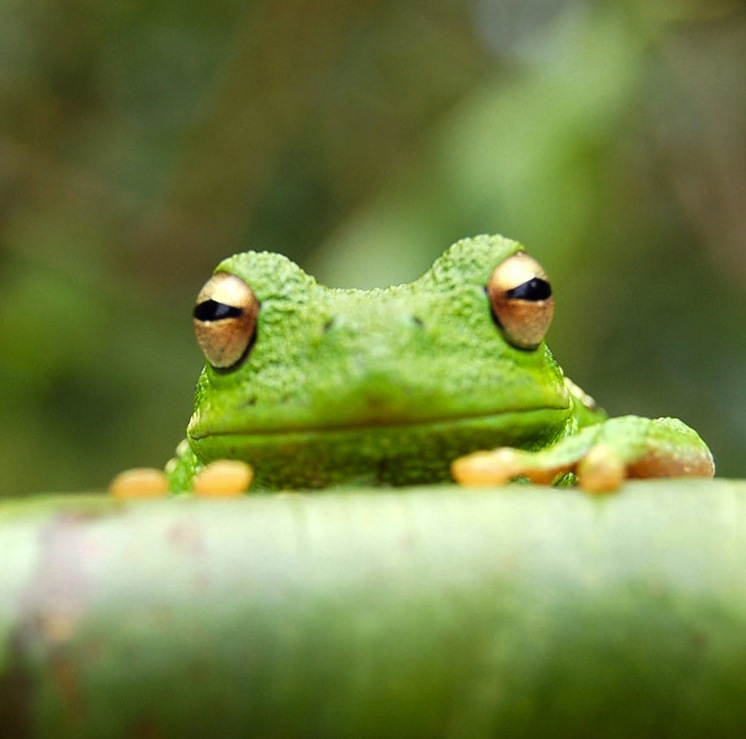
\includegraphics[width=0.3\textwidth]{frog.jpg}
\caption{\label{fig:frog}This frog was uploaded to writeLaTeX via the project menu.}
\end{figure}

\subsection{How to Make Tables}

Use the table and tabular commands for basic tables --- see Table~\ref{tab:widgets}, for example.

\begin{table}
\centering
\begin{tabular}{l|r}
Item & Quantity \\\hline
Widgets & 42 \\
Gadgets & 13
\end{tabular}
\caption{\label{tab:widgets}An example table.}
\end{table}

\subsection{How to Write Mathematics}

\LaTeX {}{} is great at typesetting mathematics. Let $X_1, X_2, \ldots, X_n$ be a sequence of independent and identically distributed random variables with $\text{E}[X_i] = \mu$ and $\text{Var}[X_i] = \sigma^2 < \infty$, and let
$$S_n = \frac{X_1 + X_2 + \cdots + X_n}{n}
      = \frac{1}{n}\sum_{i}^{n} X_i$$
denote their mean. Then as $n$ approaches infinity, the random variables $\sqrt{n}(S_n - \mu)$ converge in distribution to a normal $\mathcal{N}(0, \sigma^2)$.

\subsection{How to Make Sections and Subsections}

Use section and subsection commands to organize your document. \LaTeX {}{} handles all the formatting and numbering automatically. Use ref and label commands for cross-references.

\subsection{How to Make Lists}

You can make lists with automatic numbering \dots

\begin{enumerate}
\item Like this,
\item and like this.
\end{enumerate}
\dots or bullet points \dots
\begin{itemize}
\item Like this,
\item and like this.
\end{itemize}
\dots or with words and descriptions \dots
\begin{description}
\item[Word] Definition
\item[Concept] Explanation
\item[Idea] Text
\end{description}

\bigskip

I hope this document and the associated template package is helpful for you.  Good luck.
- Ted C. Munger

\end{document}